% This is samplepaper.tex, a sample chapter demonstrating the
% LLNCS macro package for Springer Computer Science proceedings;
% Version 2.20 of 2017/10/04
%
\documentclass[runningheads]{llncs}
%
\usepackage{float}
\usepackage{subcaption}
\usepackage[hyphens]{url}
\usepackage{hyperref}
\hypersetup{breaklinks=true}
\usepackage{graphicx}
% Used for displaying a sample figure. If possible, figure files should
% be included in EPS format.
%
% If you use the hyperref package, please uncomment the following line
% to display URLs in blue roman font according to Springer's eBook style:
% \renewcommand\UrlFont{\color{blue}\rmfamily}

\begin{document}
%
\title{Credit risk data analysis}
%
%\titlerunning{Abbreviated paper title}
% If the paper title is too long for the running head, you can set
% an abbreviated paper title here
%
\author{Kevin Attila Hartyányi\inst{C0S0RJ}}
%
%\authorrunning{F. Author et al.}
% First names are abbreviated in the running head.
% If there are more than two authors, 'et al.' is used.
%
\institute{Eötvös Loránd University, Budapest, Egyetem tér 1-3, 1053, Hungary}
%
\maketitle              % typeset the header of the contribution
%
\begin{abstract}
Classification and clustering on customer credit risk data.

\keywords{SVM  \and PCA \and KMeans \and Classification \and Clustering \and Frequent Itemsets.}
\end{abstract}
%
%
%
\section{Introduction}
In this paper I'm going to describe how I solved the assignment for the Introduction to Data Science Lecture. We will go step-by-step on the process I used to analyze, classify and cluster the data, which is about customer credit risks, and I will show the results along the way with various plots to gain more insight.

\section{Understanding the data}
As a first step we need to understand our data. This is probably the most important step as it could give us a lot of information that we can use in later phases to improve our results and save time.

The data contains categorical and numerical column. Let's take a look at the numerical data first.

\subsection{Numerical data analysis}

We first check the data distribution of the numerical values. The plotted histograms can be seen on Figure~\ref{num_data}. Here we can see that some of the histograms share a similar distribution, for example X05 and X13 or X08 and X11.

\begin{figure}[h]
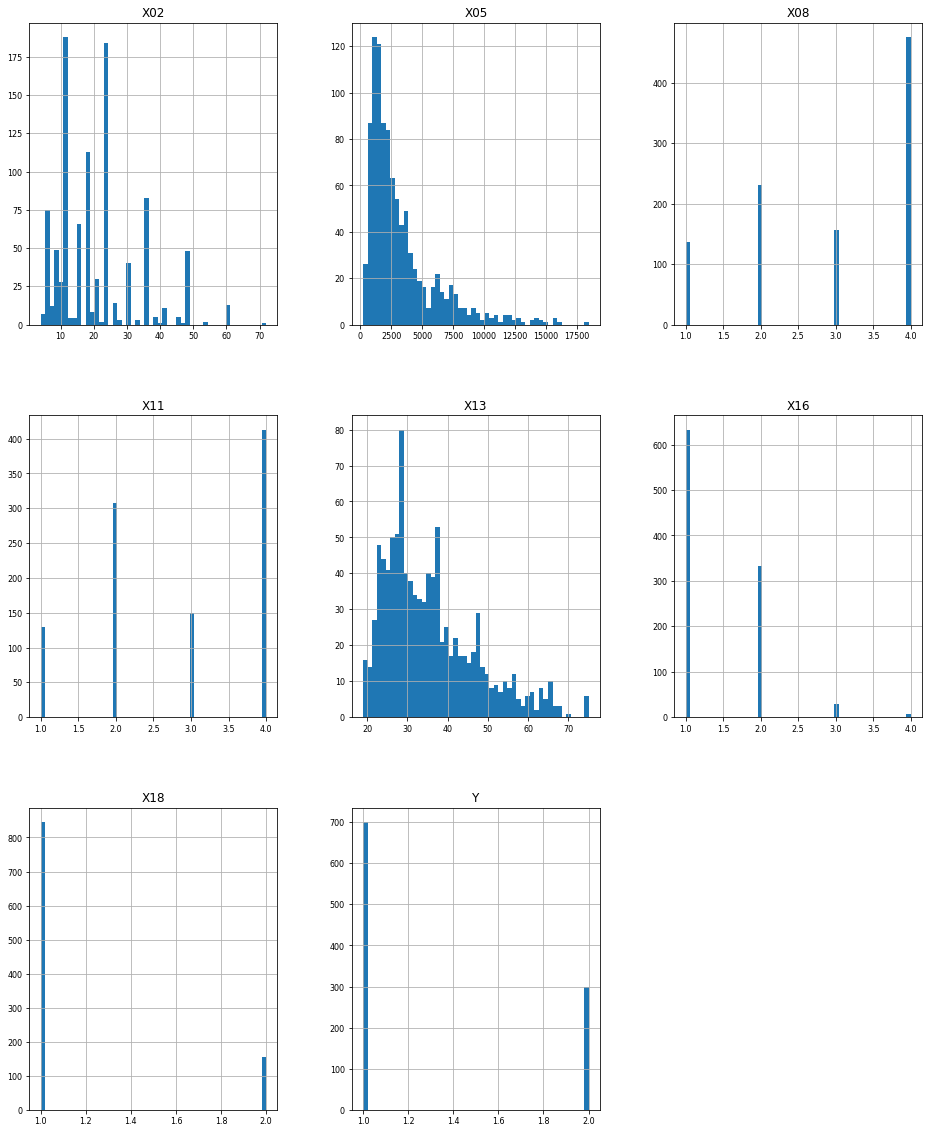
\includegraphics[width=8cm]{images/num_data.png}
\centering
\caption{Plots showing the distributions of the columns containing numerical data. We can see that some columns share a similar distribution.}
\label{num_data}
\end{figure}

We can also study the correlation matrix of these values as seen on Figure~\ref{correllation}. We are mainly interested in the Y column since that contains the information if a customer is good or bad, however even X02 which has the highest correlation with it's 0.214 value is not considered to be high.

\begin{figure}
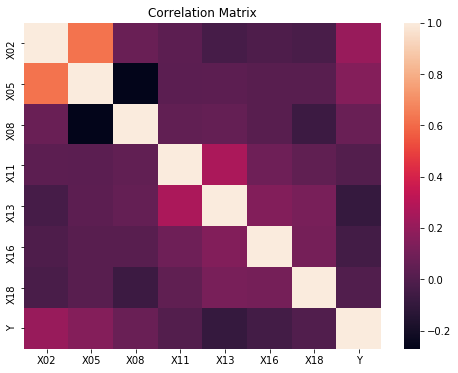
\includegraphics[width=8cm]{images/correllation.png}
\centering
\caption{Correlation matrix of the numerical data columns. We are mainly interested in the Y column as that contains the labels for the customers, it has the biggest correlation with the X02 column with a correlation number of 0.214.}
\label{correllation}
\end{figure}

\subsection{Categorical data analysis}

Now we take a look at the categorical data. We are interested in using the categorical data to find frequent itemsets in the dataset. To achieve this we use the apriori \cite{apriori} algorithm with a minimum support of 0.7. The results can be seen on Figure~\ref{apriori}. We see that almost every customer is a foreign worker in the dataset (A201). Also, 70\% of the customers are labeled as good, we need to take this into account during the training as the models might have some bias towards predicting good customers, given that the data contains a lot more examples for them. 

\begin{figure}
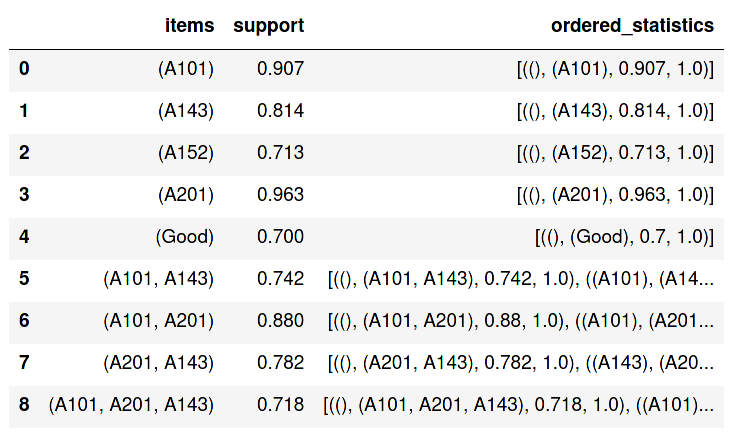
\includegraphics[width=8cm]{images/frequent_items.png}
\centering
\caption{Results of the apriori algorithm on the categorical data columns with a minimum support of 0.7.}
\label{apriori}
\end{figure}

\section{Data Preprocessing}

Now that we understand the data we need to prepare it for the models.

\subsection{Normalization}
Right now our numerical data have different scales which might end up creating a bias in the model, so we need to transform it to comparable scales that can prevent this problem. For this we can use sklearn's scale method \cite{sklearn_scale}, which center's the data to the mean and scales it to unit variance.

\subsection{Encoding}
We have dealt with the numerical columns of the data, but we still have the categorical columns left. We can't feed them to the models as they are, so we need to transform them. For this transformation we can use one hot encoding \cite{sklearn_one_hot_encoder}, which encodes our categories as one-hot numeric arrays.

The preprocessed data can be seen on Figure~\ref{processed_data}.

\begin{figure}
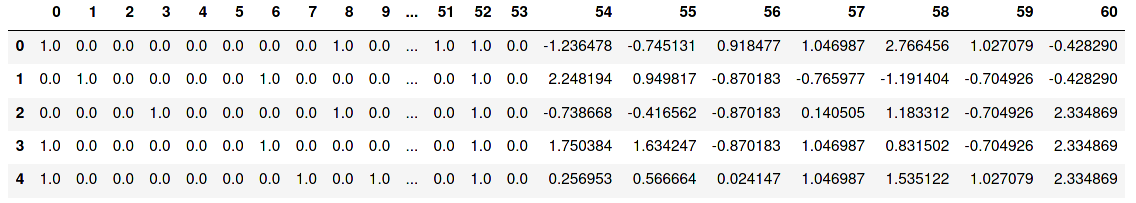
\includegraphics[width=\textwidth]{images/processed_data.png}
\centering
\caption{The customer credit data after the preprocessing. On the left side we see that the categorical columns have been transformed to one hot vectors, while on the right we see that the numerical columns have been normalized. It doesn't include the Y column that contains the labels, because that has to remain unchanged.}
\label{processed_data}
\end{figure}

\section{Classification}

We first split the data into train and test set, then we can use support vector machines \cite{sklearn_svm} for the classification of good/bad customers. 

With this setup we get a score of \textbf{0.76363}. After doing cross-validation on this model with 10 folds the results show a mean of \textbf{0.763} and a standard deviation of \textbf{0.0494}.

Looking at the classification report \ref{svm_simple} we can see that the model gets a high precision and recall for the good customer classification. However we have a constraint that we didn't take into account yet, that it is five times worse to classify customers as good when they are bad than it is to classify customers as bad when they are good. 

To satisfy this constraint we need to improve the recall of class 2 (which represents the bad customers).

\subsection{Grid Search}

To improve the recall we can do a grid search where we specify a scoring based on the recall of class 2, so the search will find an optimal parameter combination that maximizes this recall.

We can see the results of the best model after the grid search on Figure~\ref{grid_svm}. There is also a comparison between the two models plotting the precision-recall curves on Figure \ref{svm_prec_recall_plot}. We see that the recall has improved by almost 10\%, but we can do better than this.


\begin{figure}
  \centering
  \begin{subfigure}[b]{0.49\textwidth}
    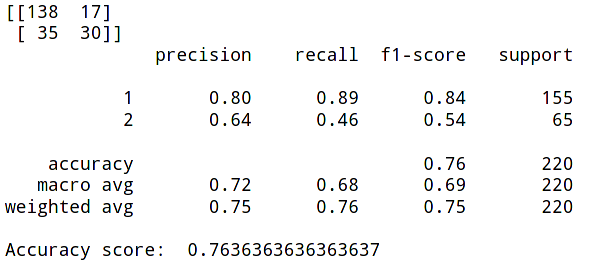
\includegraphics[width=\textwidth]{images/svm_simple.png}
    \caption{Optimized for accuracy.}
    \label{svm_simple}
  \end{subfigure}
  \hfill
  \begin{subfigure}[b]{0.49\textwidth}
    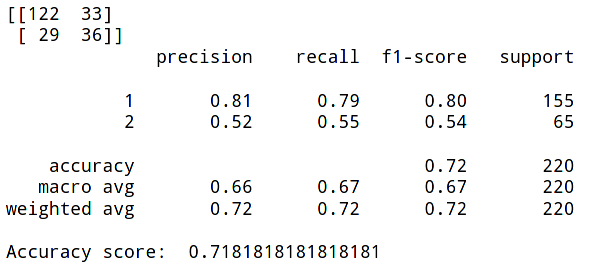
\includegraphics[width=\textwidth]{images/svm_grid.png}
    \caption{Optimized for class 2 recall.}
    \label{grid_svm}
  \end{subfigure}
  \caption{Classification report for the SVM model optimized with grid search. The recall optimized model improved the class 2 recall by 9\% while losing 5\% on average accuracy. In our case this is beneficial for us, given our constraint for the task.}
\end{figure}

\begin{figure}
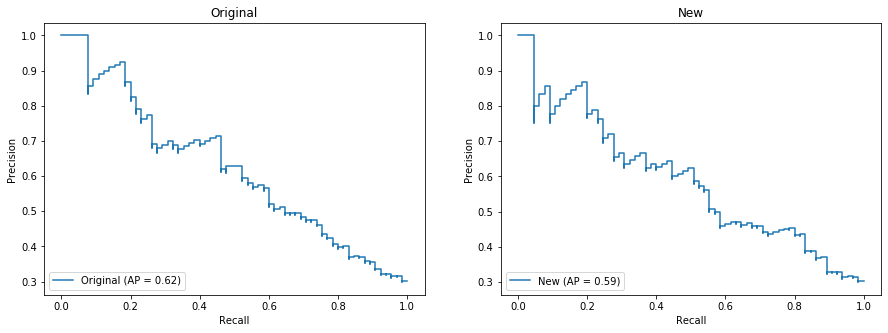
\includegraphics[width=\textwidth]{images/svm_prec_recall_comp_plot.png}
\centering
\caption{Comparison of the precision-recall curves between the original (left) and grid search optimized for recall model (right). We see that the precision on the right side shrank in favour of a higher recall}
\label{svm_prec_recall_plot}
\end{figure}


\subsection{Adjusting the probabilities of the model}
Instead of retraining we can take the probabilities of the model that it predicts for each customer. When we have these probabilities we can adjust the amount that we want for each class. In our case, we will adjust the probability of classifying a customer as good, so it requires a probability of at least 80\%, if it's smaller than this, then we classify them as bad customers. The results of this adjusted model can be seen on Figure~\ref{svm_adjusted}. 

We can see that we improved the class 2 recall of the original model by 32\% and the grid search model by 23\%. However, we did lose more than 15\% on average accuracy of the model, but given our constraint this model is more beneficial for us.

\begin{figure}
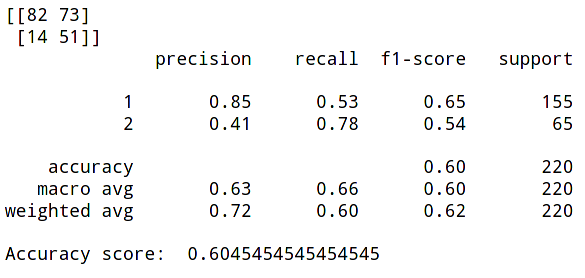
\includegraphics[width=8cm]{images/svm_adjusted.png}
\centering
\caption{Classification report for the SVM model whose probabilities have been adjusted and requires at least 80\% to classify a customer as good. The class 2 recall is greatly imrpoved compared to the previous SVM models.}
\label{svm_adjusted}
\end{figure}


\section{Principal Component Analysis}
Right now we can't easily plot our data, because it has a high dimensionality. To solve this problem we can use principal component analysis \cite{sklearn_pca} to reduce the dimensionality of the data to 2 dimensions. 

Now we can plot the data as seen on Figure~\ref{pca}. We don't see an easy way to separate the different labeled customers, but let's see if our model can find one.

\begin{figure}[h]
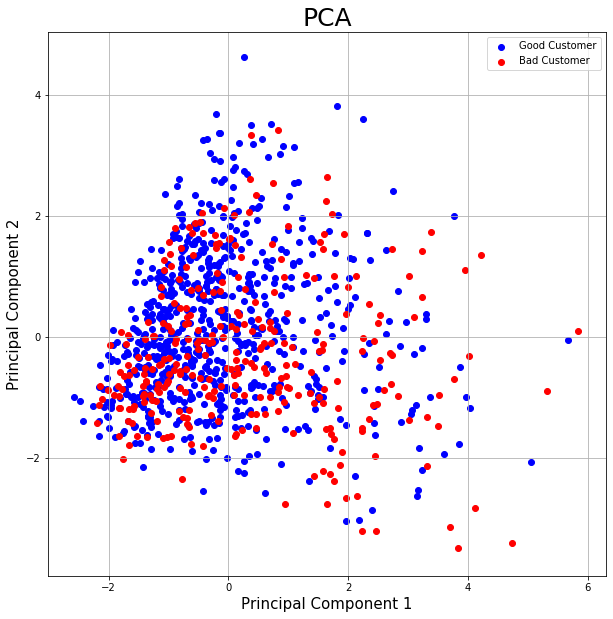
\includegraphics[width=8cm]{images/pca.png}
\centering
\caption{Data after principal component analysis. We see that most of the points are cluttered around the left side of the plot and that we can't easily see a way to separate the differently labeled points.}
\label{pca}
\end{figure}

\subsection{SVM with PCA}

Running our model with simple grid search (optimized for accuracy) on this data we get a score of \textbf{0.704} which seems nice, but after looking at the classification report Figure~\ref{svm_pca} we see that the model classified everyone as a good customer. Not really what we were looking for. We can also take a look at the plotted decision boundary of the model on Figure~\ref{svm_pca_plot} where we see that the good customer examples overwhelm the decision of the model. 


\begin{figure}
  \centering
  \begin{subfigure}[b]{0.49\textwidth}
    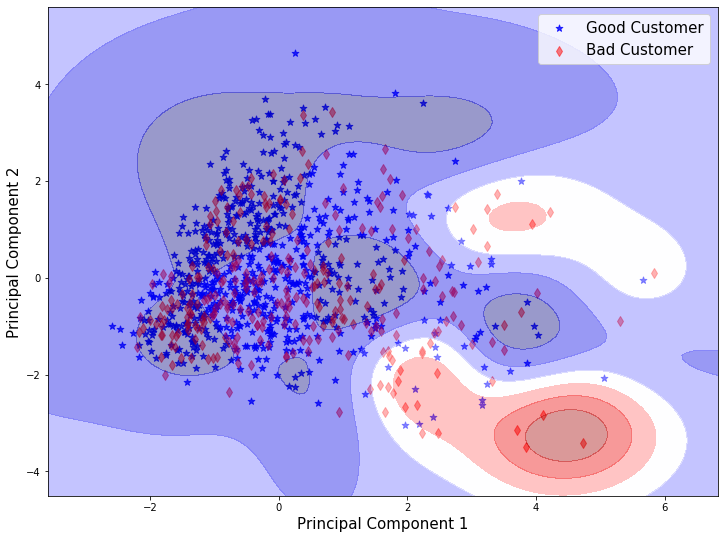
\includegraphics[width=\textwidth]{images/svm_pca_simple_plot.png}
    \caption{Optimized for accuracy.}
    \label{svm_pca_plot}
  \end{subfigure}
  \hfill
  \begin{subfigure}[b]{0.49\textwidth}
    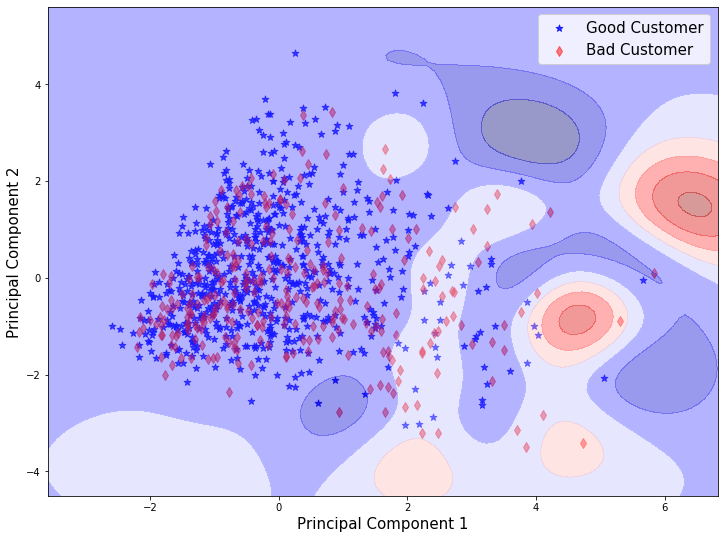
\includegraphics[width=\textwidth]{images/svm_pca_grid_recall_plot.png}
    \caption{Optimized for class 2 recall.}
    \label{svm_pca_recall_plot}
  \end{subfigure}
  \caption{Decision boundary of the svm model optimized with grid search on the dimensionality reduced data by pca. Optimizing for accuracy we see that the higher amount of good customer examples overwhelm the decision of the model predicting most customers as good. This effect can be reduced by optimizing for recall, but not to much extent.}
  \label{decision_boundary}
\end{figure}

Changing the grid search optimization score to the class 2 recall we get an accuracy of \textbf{0.709}. The classification report for this model is on Figure~\ref{svm_pca_recall} and the plot of the decision boundary is on Figure~\ref{svm_pca_recall_plot}. This achieves somewhat better results, but still far from what we have achieved on the original data.


\begin{figure}[h]
  \centering
  \begin{subfigure}[b]{0.49\textwidth}
    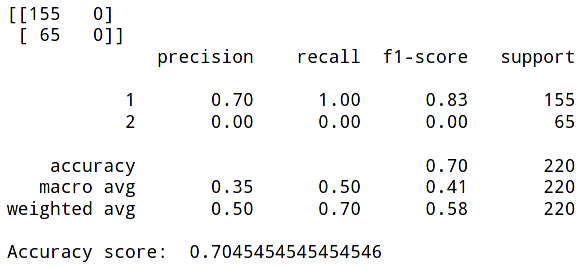
\includegraphics[width=\textwidth]{images/svm_pca_simple.png}
    \caption{Optimized for accuracy.}
    \label{svm_pca}
  \end{subfigure}
  \hfill
  \begin{subfigure}[b]{0.49\textwidth}
    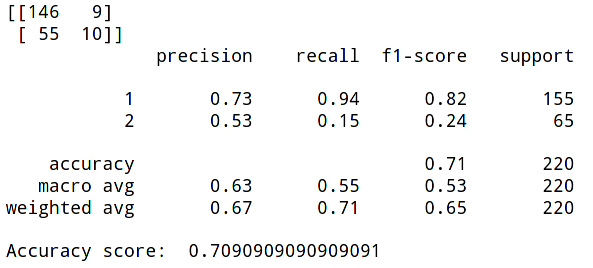
\includegraphics[width=\textwidth]{images/svm_pca_grid_recall.png}
    \caption{Optimized for class 2 recall.}
    \label{svm_pca_recall}
  \end{subfigure}
  \caption{Classification report for the SVM model trained on the dimesnionality reduced data by pca and optimized with grid search. As discussed on Figure~\ref{decision_boundary} the accuracy optimized model predicts all examples as good customers.}
\end{figure}


\section{Clustering}
\subsection{KMeans}
We can use KMeans for clustering the customers into various groups. Let's first see how well the model performs when we use a cluster number of 2 to classify the customers to be good/bad without the labels. The classification report Figure~\ref{kmeans} showed an accuracy of \textbf{0.664}, which is not that bad given that it did all of this unsupervised.

If we didn't have the labels for the customers we wouldn't know how many clusters we should use, for this we can use the elbow method to estimate a good cluster number. A plot showing the elbow method on this data can be seen on Figure~\ref{kmeans_elbow}. The y axis on this plot refers to the distortion which is the sum of squared distances of samples to their closest cluster center.
We don't see any plateau on this graph so it's not easy to choose a good cluster number.

\begin{figure}
  \centering
  \begin{subfigure}[b]{0.49\textwidth}
    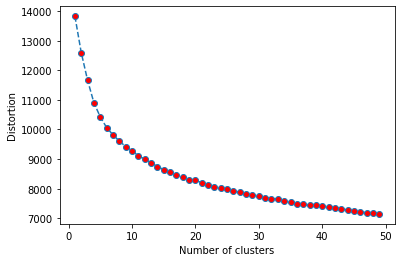
\includegraphics[width=\textwidth]{images/kmeans_elbow.png}
    \caption{On the original data.}
    \label{kmeans_elbow}
  \end{subfigure}
  \hfill
  \begin{subfigure}[b]{0.49\textwidth}
    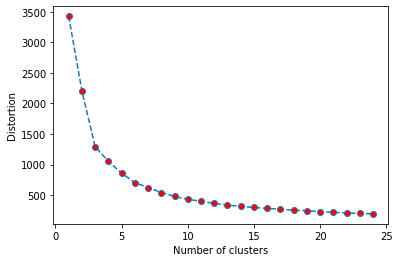
\includegraphics[width=\textwidth]{images/kmeans_pca_elbow.png}
    \caption{On the dimensionality reduced data by pca.}
    \label{kmeans_pca_elbow}
  \end{subfigure}
  \caption{Elbow method using KMeans model. On the original data the curve keeps decreasing so we can't easily find a good cluster number, while on the dimensionality reduced data we see that it starts to plateau around 20 clusters.}
\end{figure}

\subsection{KMeans with PCA}
For better visualization we can try our KMeans model on the dimensionality reduced data. On this data we achieve an accuracy of \textbf{0.662} Figure~\ref{kmeans_pca}. 

\begin{figure}
  \centering
  \begin{subfigure}[b]{0.49\textwidth}
    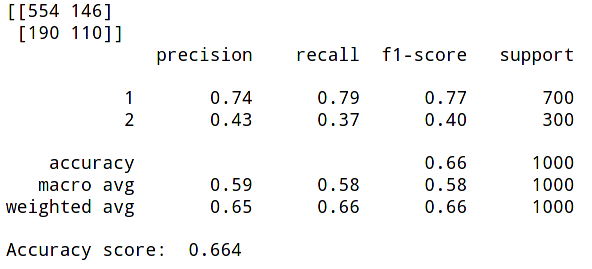
\includegraphics[width=\textwidth]{images/kmeans.png}
    \caption{On the original data.}
    \label{kmeans}
  \end{subfigure}
  \hfill
  \begin{subfigure}[b]{0.49\textwidth}
    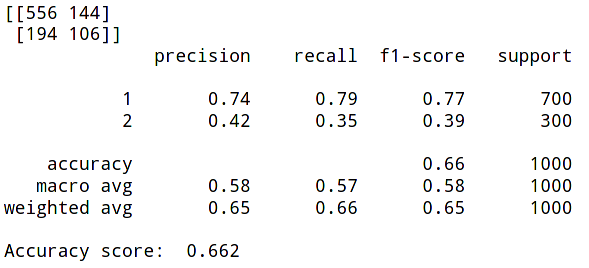
\includegraphics[width=\textwidth]{images/kmeans_pca.png}
    \caption{On the dimensionality reduced data by pca.}
    \label{kmeans_pca}
  \end{subfigure}
  \caption{Classification report for the KMeans model using 2 clusters. It receives similar results for the original and the dimesnionality reduced data.}
\end{figure}

A visualization of this clustering can be seen on Figure~\ref{kmeans_pca_plot}.

Using the elbow method again on Figure~\ref{kmeans_pca_elbow} we see a nicer graph where the cluster number distortion starts to plateau around 20 clusters. The results of clustering with this number can be seen on Figure~\ref{kmeans_pca_optim_cluster}.

\begin{figure}[h]
  \centering
  \begin{subfigure}[b]{0.49\textwidth}
    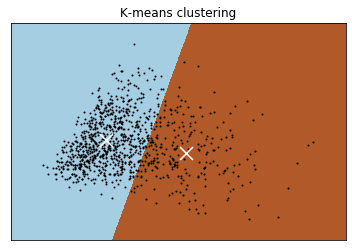
\includegraphics[width=\textwidth]{images/kmeans_pca_plot.png}
    \caption{Using 2 clusters. Good/bad customers.}
    \label{kmeans_pca_plot}
  \end{subfigure}
  \hfill
  \begin{subfigure}[b]{0.49\textwidth}
    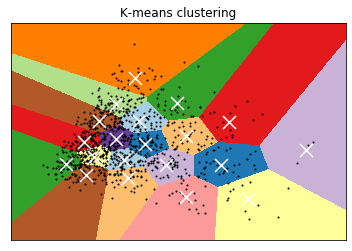
\includegraphics[width=\textwidth]{images/kmeans_pca_optim_cluster.png}
    \caption{Using 20 clusters. We use 20 clusters, because the elbow method on this data starts to plateau around this point.}
    \label{kmeans_pca_optim_cluster}
  \end{subfigure}
  \caption{Visualization of the KMeans model with different clusters on the dimensionality reduced data by pca.}
\end{figure}

\section{Conclusion}

We have tried SVM, PCA and KMeans with different parameters on the customer credit data.

With the SVM we achieved an accuracy of \textbf{0.763} with a class 2 recall of \textbf{0.46}, which after taking the constraint of the task into account was reduced to \textbf{0.604}, but with the much better class 2 recall of \textbf{0.78}. 

We used PCA for dimensionality reduction, so we could visualize the data. We also tried this data with SVM and KMeans, with the purpose of finding something interesting and to understand the data better.

For clustering the customers into various groups we used KMeans. We were able to estimate the accuracy of the clustering when we created 2 clusters from the data \textbf{0.662}, because we had the labels for them, however most of the time we don't have labels for our data, so we also checked other methods, like the elbow technique for deciding what is a nice cluster number for the data.


% ---- Bibliography ----
%
% BibTeX users should specify bibliography style 'splncs04'.
% References will then be sorted and formatted in the correct style.
%
% \bibliographystyle{splncs04}
% \bibliography{mybibliography}
%
\begin{thebibliography}{8}
\bibitem{sklearn_scale}
Sklearn Scale, \url{https://scikit-learn.org/stable/modules/generated/sklearn.preprocessing.scale.html}. Last accessed 4 Dec 2020


\bibitem{sklearn_one_hot_encoder}
Sklearn OneHotEncoder, \url{https://scikit-learn.org/stable/modules/generated/sklearn.preprocessing.OneHotEncoder.html}. Last accessed 4 Dec 2020

\bibitem{sklearn_svm}
Sklearn SVM, \url{https://scikit-learn.org/stable/modules/generated/sklearn.svm.SVC.html}. Last accessed 4 Dec 2020

\bibitem{sklearn_pca}
Sklearn PCA, \url{https://scikit-learn.org/stable/modules/generated/sklearn.decomposition.PCA.html}. Last accessed 4 Dec 2020

\bibitem{sklearn_kmeans}
Sklearn KMeans, \url{https://scikit-learn.org/stable/modules/generated/sklearn.cluster.KMeans.html}. Last accessed 4 Dec 2020

\bibitem{pca_boundary}
PCA Boundary visualization, \url{https://towardsdatascience.com/visualizing-support-vector-machine-decision-boundary-69e7591dacea}. Last accessed 4 Dec 2020

\bibitem{apriori}
Apriori algorithm implementation, \url{https://pypi.org/project/apyori/}. Last accessed 4 Dec 2020

\end{thebibliography}
\end{document}
